In this section we will discuss about the whole approach to identify the hyper-
giants presence in today's Internet.The key idea is to collect IP addresses that
DNS returns for Alexa top 100,000 websites and the website links embedded in
these top 100,000 websites.We will use the content type of all the HTTP request
and find out the different object type (text/html,image,video,audio etc) delivered by these hyper giants for the popular websites and the embedded links in
those websites.

\begin{figure}[h]
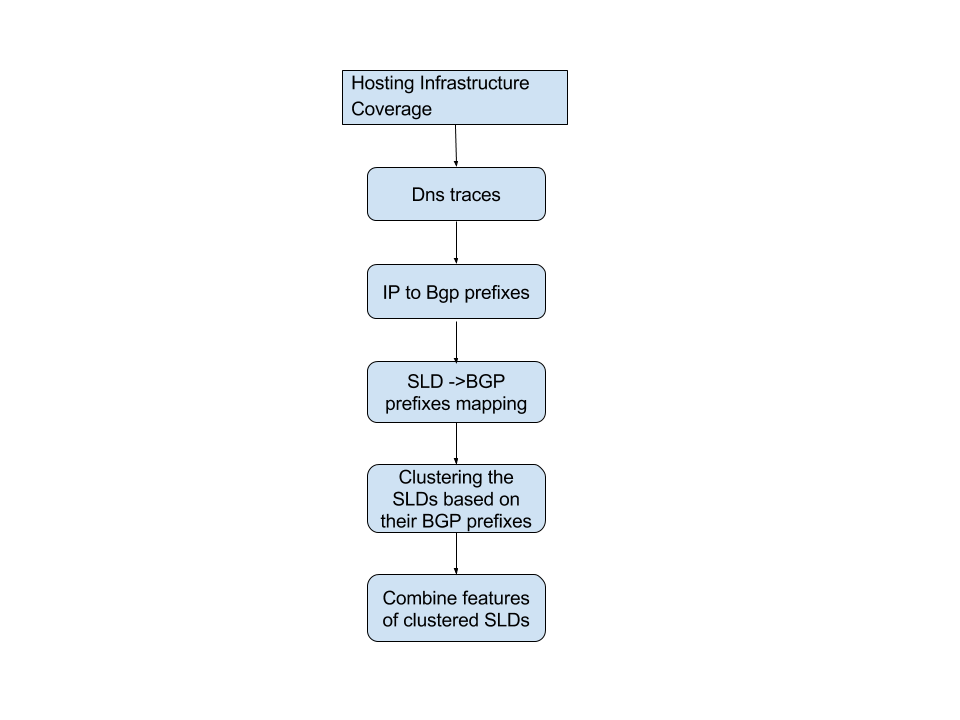
\includegraphics[width=\textwidth,height=10cm]{/home/sakib/soumya/wholeSLD/High Level Of Approach.png}
\centering
\caption{High Level Of Approach}
\end{figure}

To achieve our goals of identifying and classifying hyper giants in Internet,we
divided the whole process into 6 parts shown in figure 6.We now elaborate the
steps we followed ,choices we have taken to achieve our goals.

\subsection{Hosting Infrastructure Coverage}
To achieve our goals to find out the hyper giants in Internet,we will use the SLD infrastructures which are serving popular websites.Given that Internet traffic
normally consistent with the Zipf’s law [22],it is very likely possible that the hyper giants are the very popular content delivery networks or content providers
etc. which are responsible for the majority of the HTTP traffic flow in today's
Internet.For example, Akamai claims to deliver about 20\% of the total Web
traffic in the Internet [5]. According to Labovitz et al. [2] ,Google serves up to
10 \% of all Internet traffic.Similarly top 10 hosting infrastructures serve more
than 15\% and top 100 responsible for more than 40\% of the traffic.In this thesis
we will take the Alexa top 100,000 popular websites/
\subsection{DNS traces}
We base our study on DNS traces collected within single vantage point within
Germany.So this thesis will provide a better overview of hyper giants behavior
within our vantage point location in Germany.As hyper giants are normally vast
hosting infrastructures,content providers etc. ,their footprint mostly present all
over the world .Hence the identification of hyper giants should not be affected
much due to this limitation.But there are few other research questions arises
due to this network coverage limitation .We will discuss about these
research questions in "Future Work" chapter.For collecting data we use ”Scrapy”
framework.Scrapy framework is an open source web crawler.
\subsection{IP to BGP Prefixes Mapping}

\begin{figure}[h]
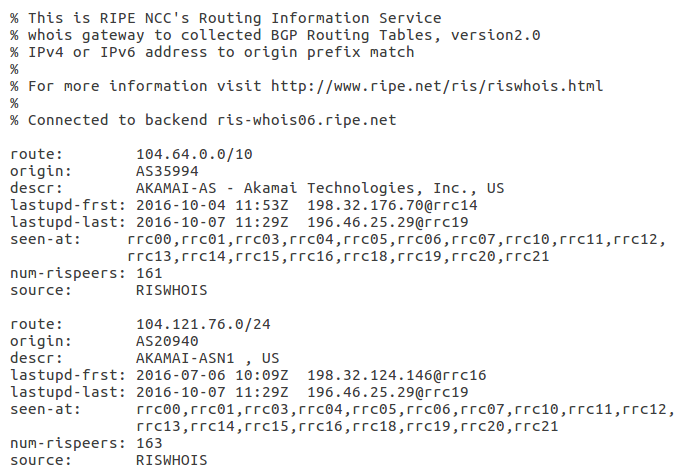
\includegraphics[width=\textwidth,height=10cm]{/home/sakib/soumya/latexNew/whois.png}
\centering
\caption{RIPE RIS bgp prefixes using whois command}
\end{figure}

We extract IP addresses of each website link using scrapy crawler.Along with
this we also collect the ARecord names associated with the corresponding IP
address.From ARecord names we collect the SLDs.The set of IP addresses for a
perticular SLD shows the degree to which the corresponding SLD infrastructure
is network-wise and geographically distributed.Hence natural choice for the features to consider are IP addresses,AS Numbers and the bgp prefixes.The number
of bgp prefixes shows the network footprint and the number of ASNs shows how
infrastructures are distributed all over the world.For example the highly distributed
infrastructures have a lot of prefixes as well as high number of ASNs.Similarly
small data centers will be located within a single AS , having a limited number of bgp prefixes,and a large number of IP addresses.Eventually these features are correlated and using these features we will try to find out the hyper giants presence in Internet.
To determine bgp prefixes we use BGP routing information from RIPE RIS[23].The bgp prefix information for IP address 104.121.76.73 is shown in the
figure 7.As we can see from figure-7, the information provided are like routes
which is the bgp prefixes,origin shows the corresponding AS number.From the
figure this can be seen that the ip address 104.121.76.73 can be routed via two
different prefixes 104.64.0.0/10 and 104.121.76.0/24.So we will consider both the
prefixes for the IP address 104.121.76.73.
\subsection{SLD to BGP Mapping}
From the second stage shown in figure-6,we receive IP address and corresponding
ARecords.From the ARecord,we get second level domain which gives us idea
about the infrastructure involved with the website.Again from stage-3 shown in figure-6 ,we get
the IP address to BGP prefixes mapping using RIPE RIS bgp prefixes.In this stage we will
create the mapping of SLD infrastructures collected in stage -2 shown in figure-6 to BGP prefixes
collected in stage-3 shown in figure-6.Now we have all features IP addresses,BGP prefixes,ASN
numbers which are required for determining the type of infrastructure.
\subsection{Clustering Algorithm}
The clustering algorithm can be divide into two parts.In the first step ,we will
try to aggregate the prefixes of a SLD into the set of parent prefixes and in
the subsequent step we will compare prefixes of the SLDs with each other and
cluster them if they are sharing most of the infrastructures.
\subsubsection{Aggregate Prefixes}
From the above steps,we collected SLDs with corresponding number of links
served by SLD,number of IP addresses,bgp prefixes and number of ASNs.Now
first we will sort the SLDs according to their number of links in decreasing or-
der.This will give us all the popular SLDs which served maximum number of
links.Now from the bgp prefixes,keep only parent prefixes and the prefixes which
do not have any child in the prefix set.for example, googledomains.com has the
prefix set (’216.239.32.0/19’, ’216.239.32.0/24’, ’216.239.34.0/24’, ’216.239.36.0/24’),
’216.239.38.0/24’).After the above step the prefix set will become (’216.239.32.0/19’])
as other prefixes are subset of parent prefix 216.239.32.0/19.This procedure will
be done for all the SLDs staring from first SLD sorted by decreasing order of
number of links.Now starting from first and compare each SLD with the other
SLDs.Between two prefix sets if child prefixes present then replace with parent
prefix.This will make two prefix set with only parents.Now compare the two sets
of prefixes to find out whether they are sharing same infrastructure or not.More
details about the similarity procedure will be discussed in the next section.
\subsubsection{Similarity between two prefixes set}
Based on the similarity between two prefix set,we will decide if they belong to
same SLD infrastructure or not.For this we define the similarity between two
prefix set as follows,
\begin{equation}
similarity(s1, s2)= \frac{|s1 \cap s2|}{|s2|}
\end{equation}

where s1,s2 are the bgp prefix sets.

If the similarity between two prefix sets are greater than equal to 70\% then
we cluster both the SLDs together.Here we assume than if s2’s 70\% prefixes
are present in the common infrastructure between s1 and s2 set,then it shows
that s2 sharing most of the infrastructure of s1.Hence we club them together.We
will continue this procedure for all the SLDs starting from the first SLD sorted
by their number of links. If two SLDs are matched ,they it will be removed from
comparison with other SLDs and it will be mapped to the SLD with which it
matched.For example ’googleusercontent.com’ matched with ’google.com’ with
similarity 100\%.Once this is matched we clubbed googleusercontent.com with
google.com and will not be available for any further similarity matching with other SLDs.70\%
of similarity is chosen after extensively testing between bgp prefixes.But this
can be taken for future work.
\subsection{Combine features of clubbed SLDs}
Now after the cluster algorithms, we will get prominent SLD infrastructures
under which multiple number of SLD mapped to based on similarity comparison
between the bgp prefixes they routed to.Hence now we will club the features of
the child SLDs with the parent SLDs.After this stage we have all the prominent
infrastructures with number of unique bgp prefixes by both parent SLD and child
SLDs,unique links by both parent SLD links and child SLDs ,unique ASNs both
parent SLD links and child SLDs.
\subsection{Conclusion}
In this section we discussed about the whole method we are going to follow to
reach our goals.Along with this we identify some of the future works which will
be discussed briefly in ”Future work” section.